%%%%%%%%%%%%%%%%%%%%%%%%%%%%%%%%%%%%%%%%%%%%%%%%%%%%%%%
% % Lines starting with % are comments, which are ignored.
% % This is a handy way of indicating the date and version of
% % your document, to wit:
% %
% % LaTeX sample file
% % Modified March, 2002
% %
%%%%%%%%%%%%%%%%%%%%%%%%%%%%%%%%%%%%%%%%%%%%%%%%%%%%%%%
\DocumentMetadata{
  % PDF standards: ONE key whose value is a comma-separated list --
  % UA-2 (accessibility) plus A-4f (archival; the archival companion of
  % UA-2). Do NOT use separate pdfstandard=... keys: with ordinary
  % key-value parsing only the last one takes effect.
  pdfstandard={UA-2,A-4f},
  lang=en-US,
  tagging=on,
  tagging-setup={
    math/setup=mathml-SE
  }
}

\documentclass[12pt]{exam}
% worksheet-macros.tex -- shared package setup for worksheet-template.tex.
%
% NOTE ON PATHS: every template in this repository is stored one level up
% from where it is compiled (see README.md). All relative \input paths
% below are resolved against the folder the document is compiled in,
% which sits one directory above this file.

% --- Math ------------------------------------------------------------
% amsmath: equation environments and numbering
% amsfonts: \mathbb etc.  |  mathrsfs: \mathfrak  |  stmaryrd: extra symbols
\usepackage{amsmath}
\usepackage{amsfonts}
\usepackage{mathrsfs}
\usepackage{stmaryrd}

% --- Layout and glyphs ------------------------------------------------
% float: [H] float placement (stop floats where you put them)
% fontspec: Unicode/OpenType fonts (compile with XeLaTeX or LuaLaTeX)
% emoji: emoji glyphs in the text
\usepackage{float}
\usepackage{fontspec}
\usepackage{emoji}

% --- Typography --------------------------------------------------------
% Atkinson Hyperlegible as the document-wide sans serif (sfdefault):
% a high-legibility face that is easier to read for students with
% dyslexia or low vision.
\usepackage[sfdefault]{atkinson}

% --- Colors -------------------------------------------------------------
% dvipsnames: extended named color palette (the Accessible* colors in
%   lecture-macros.tex are built on it);
% table: \rowcolors / \cellcolor for shading worksheet tables.
% NOTE: xcolor may only be loaded ONCE per document -- a second
% \usepackage{xcolor} with different options is a fatal "Option clash"
% error, so ALL of its options are listed here.
\usepackage[dvipsnames,table]{xcolor}

% --- Multimedia ---------------------------------------------------------
% animate: embeds audio/video (and legacy Flash) media in the worksheet.
\usepackage{animate}

% --- Bibliography --------------------------------------------------------
% biblatex (biber backend): citations and a reference list for worksheets.
\usepackage[
  backend=biber,
  style=alphabetic,
  url=true,
  doi=true,
  isbn=true,
  backref=true
]{biblatex}

% --- Links ---------------------------------------------------------------
% hyperref makes every \ref/citation/URL clickable in the PDF.
% Link colors must satisfy WCAG 1.4.3 (>= 4.5:1 contrast on white):
%   blue = 8.6:1, green!40!black = 7.2:1.
% (The old cyan/magenta values measured 1.25:1 / 3.1:1 and failed.)
\usepackage{hyperref}
\hypersetup{
  colorlinks=true,
  linkcolor=blue,
  filecolor=blue,
  urlcolor=green!40!black,
}

% --- Shared course macros ------------------------------------------------
% Root macros.tex: math shorthands used across all course documents
% (\RR, \NN, \ZZ, \QQ, \grad, \curl, \tr, \der, \pder, ...).
\newcommand{\RR}{\mathbb{R}}
\newcommand{\NN}{\mathbb{N}}
\newcommand{\ZZ}{\mathbb{Z}}
\newcommand{\QQ}{\mathbb{Q}}
\newcommand{\vv}{\vec{v}}
\newcommand{\ww}{\vec{w}}
\newcommand{\xx}{\vec{x}}
\newcommand{\yy}{\vec{y}}
\newcommand{\zz}{\vec{z}}
\newcommand{\uu}{\vec{u}}
\newcommand{\basis}[1]{\vec{e_{#1}}}
\newcommand{\id}{\mathrm{id}}
\newcommand{\CC}{\mathbb{C}}
\renewcommand{\div}{\operatorname{div}}
\newcommand{\grad}{\operatorname{grad}}
\newcommand{\curl}{\operatorname{curl}}
\newcommand{\tr}{\operatorname{tr}}
\newcommand{\der}[2]{\dfrac{d #1}{d #2}}
\newcommand{\pder}[3][]{\dfrac{\partial^{#1} #2}{\partial #3}}


% % Title and author(s)
%%%%%%%%%%%%%%%%%%%%%%%%%%%%%%%%%%%%%%%%%%%%%%%%%%%%%%%
\title{Worksheet 14: L'Hôpital's Rule}
\author{MATH 1271}
\date{10/27/2026}
%%%%%%%%%%%%%%%%%%%%%%%%%%%%%%%%%%%%%%%%%%%%%%%%%%%%%%%
% %
% % The next command allows your in import encapsulated
% % postscript files, .epsf or .eps files, which
% % contain vector graphic image data.
% %
%%%%%%%%%%%%%%%%%%%%%%%%%%%%%%%%%%%%%%%%%%%%%%%%%%%%%%%
% %   The first thanks indicates your affiliation
% %
% %  Just the name here.
% %
% % Your mailing address goes at the end.
% %
% % \thanks is also how you indicate grant support
% %
%%%%%%%%%%%%%%%%%%%%%%%%%%%%%%%%%%%%%%%%%%%%%%%%%%%%%%%

%%%%%%%%%%%%%%%%%%%%%%%%%%%%%%%%%%%%%%%%%%%%%%%%%%%%%%%
% $ The next command ensures the margins are 1 inch on
% % all sides.
% %
%%%%%%%%%%%%%%%%%%%%%%%%%%%%%%%%%%%%%%%%%%%%%%%%%%%%%%%
\begin{document}
\newpage
\maketitle

\begin{enumerate}

\item For each limit below, answer the following questions:

\begin{itemize}
	\item Is the limit indeterminate?
	\item If the limit is indeterminate, is the limit of the form where you can immediately apply L'H\^opital's Rule?
	\item What is the value of the limit?
\end{itemize}	

\smallskip

\begin{enumerate}

\item $\displaystyle\lim_{x\to 0}\frac{\ln(1+x)}{x}$

\vfill

\item $\displaystyle\lim_{x\to \pi}\frac{\cos(x)}{x}$

\vfill

\item $\displaystyle\lim_{x\to0}\frac{\sin(x)-x}{\cos(2x)-1}$

\vfill

\item $\displaystyle\lim_{x\to 0^+} \frac{\ln(x)}{1/x}$

\vfill

\newpage

\item $\displaystyle\lim_{x\to \pi/2}\frac{\tan(x)}{x-\frac{\pi}{2}}$

\vspace{2.1in}

\item $\displaystyle\lim_{x\to +\infty}xe^{-10x}$

\vspace{2.1in}

\item $\displaystyle\lim_{x\to 1}\left(\frac{1}{x-1}-\frac{x}{\ln(x)}\right)$

\vfill

\end{enumerate}

\newpage

\item Three pairs of functions are graphed below:

\begin{center}
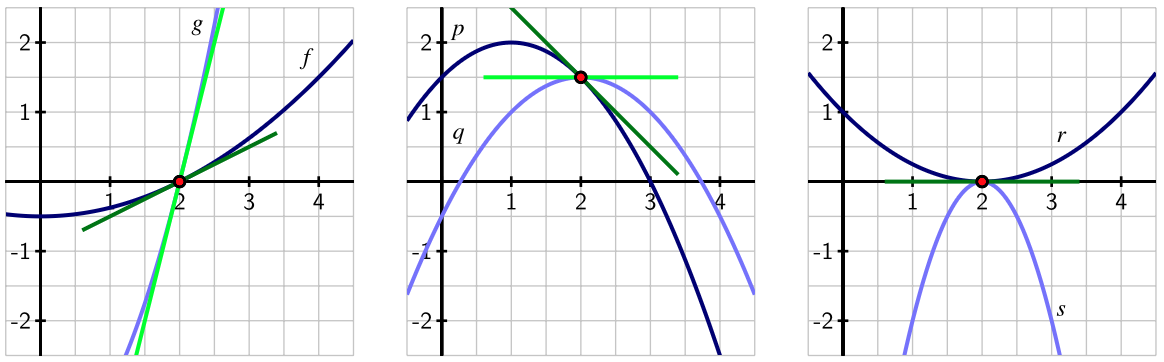
\includegraphics[scale=0.36]{wkst15graph-f25.png}
\end{center}

\begin{enumerate}

\item Use the left-hand graph to determine the values of $f(2)$, $f'(2)$, $g(2)$, and $g'(2)$. Then, evaluate $\displaystyle\lim_{x\to 2}\frac{f(x)}{g(x)}$.

\vfill

\item Use the middle graph to find $p(2)$, $p'(2)$, $q(2)$, and $q'(2)$. Then, evaluate $\displaystyle\lim_{x\to 2}\frac{p(x)}{q(x)}$.

\vfill

\item Assume that $r$ and $s$ are functions for which $r''(2)\neq0$ and $s''(2)\neq0$. Use the right-hand graph to compute $r(2)$, $r'(2)$, $s(2)$, and $s'(2)$. Explain why you cannot determine the exact value of $\displaystyle\lim_{x\to 2}\frac{r(x)}{s(x)}$ without further information being provided, but that you can determine the sign of $\displaystyle\lim_{x\to 2}\frac{r(x)}{s(x)}$. State what the sign of the limit will be (with justification).

\vfill

\end{enumerate}

\newpage

\item \textbf{The Ultraviolet Catastrophe}: Before the advent of quantum mechanics, physicists studied the amount of energy given off by a radiating mass as a function of the wavelength of light emitted by it. We can use L'Hôpital's rule to get a hands on way of seeing how quantum mechanics remedies a terrible error!

  \begin{enumerate}
    \item \textbf{The Catastrophe}: The best pre-quantum mechanics description we had for this relationship between energy and wavelength
      was the Rayleigh-Jeans Law:
      \begin{equation}
        B_{RJ}(\lambda) = \dfrac{K}{\lambda^4}
      \end{equation}
      where $\lambda$ is the wavelength of light, and $K$ is the \textit{Boltzmann constant}.
      We call light that has a very small wavelength ultraviolet.
      Analyze the limit of the above function as $\lambda \rightarrow 0$
      and use what you find to argue whether or not
      that function provides an accurate model for real world ultraviolet behavior. 
      \vfill

    \item \textbf{The Quantum Solution:} Maxwell Planck thought that assuming
      blackbodies could only emit highly specific energy levels of light (so called \textit{quantized} energy states) would remedy this situation,
      and used that assumption to instead model blackbody radiation as:
      \begin{equation}
        B_P(\lambda) = \frac{k_1}{\lambda^5} \dfrac{1}{e^{\frac{k_2}{\lambda}} - 1}
      \end{equation}
      where again $\lambda$ is the wavelength and $k_1, k_2$ are just some constants. Analyze the limit of this function as $\lambda \rightarrow 0$ and use what you find to argue whether or not this function provides a more accurate model of real world ultraviolet behavior than the Rayleigh-Jeans model.
      \vfill
  \end{enumerate}

\end{enumerate}

% Most people don't use these, so they are "commented out"
% by starting the lines with a "%"
%\begin{keywords}
%   \LaTeX, typesetting
%\end{keywords}

%\begin{AMS}
%   50C60, 18C25
%\end{AMS}

%%%%%%%%%%%%%%%%%%%%%%
% % Here is the start of the Text
%%%%%%%%%%%%%%%%%%%%%%
\end{document}
